\documentclass[12pt]{iopart}
\pdfminorversion=4
\usepackage{graphicx}
%Uncomment next line if AMS fonts required
%\usepackage{iopams}  
\begin{document}

\title[Electroweak phyiscs at the LHC]{Electroweak physics at the LHC}
\author{J Berryhill$^1$ and A Oh$^2$}

\address{$^1$ Fermi National Accelerator Laboratory, Batavia, IL, USA}
\address{$^2$ School of Physics and Astronomy, University of Manchester, Manchester, UK}

%\ead{submissions@iop.org}
%\vspace{10pt}
%\begin{indented}
%\item[]February 2014
%\end{indented}

\begin{abstract}
The Large Hadron Collider (LHC) has completed in 2012 its first
running phase and the experiments have collected data sets of pp
collisions at center-of-mass energies of 7 and 8 TeV with an
integrated luminosity of about 5ifb and 20ifb, respectively.  Analyses
of these data sets have produced a rich set of results in the
electroweak sector of the standard model. This article reviews the
status of electroweak measurements of the ATLAS and CMS experiments at
the LHC and discusses phenomenological developments in the electroweak
sector.
\end{abstract}

% Uncomment for PACS numbers
\pacs{00.00, 20.00, 42.10}
%
% Uncomment for keywords
\vspace{2pc}
\noindent{\it Keywords}: XXX, YYY, ZZZ
%
% Uncomment for Submitted to journal title message
\submitto{\jpg}
%
% Uncomment if a separate title page is required
\maketitle
% 
% For two-column output uncomment the next line and choose [10pt] rather than [12pt] in the \documentclass declaration
%\ioptwocol
%


\section{Introduction}
\subsection{Motivation to study the electroweak sector}
\subsection{Electroweak physics at hadron colliders}
\subsection{LHC physics program}
\subsection{Electroweak challenges for Run 2 and beyond}

\section{Theory overview and recent developments}
\subsection{PDF and electroweak observables (V+jets, phi*)}
\subsection{Electroweak NLO corrections}
\subsection{Anomalous gauge couplings and effective field theory}
\subsection{Oblique corrections, constructed observables}


\section{Inclusive boson production}
\subsection{Drell-Yan production}
ATLAS high-mass Drell--Yan 7 TeV~\cite{Aad:2013iua} 

ATLAS low-mass Drell-Yan 7 TeV~\cite{Aad:2014qja}

ATLAS Z PT 7 TeV~\cite{Aad:2014xaa}

ATLAS Z phistar 7 TeV~\cite{Aad:2012wfa}

CMS Drell--Yan 7 TeV~\cite{Chatrchyan:2013tia}

CMS Drell--Yan 8 TeV~\cite{CMS:2014jea}

CMS angular coefficients 8 TeV~\cite{Khachatryan:2015paa}

CMS Z PT and rapidity 8 TeV~\cite{Khachatryan:2015oaa}

\begin{figure}[p]
    \centering
    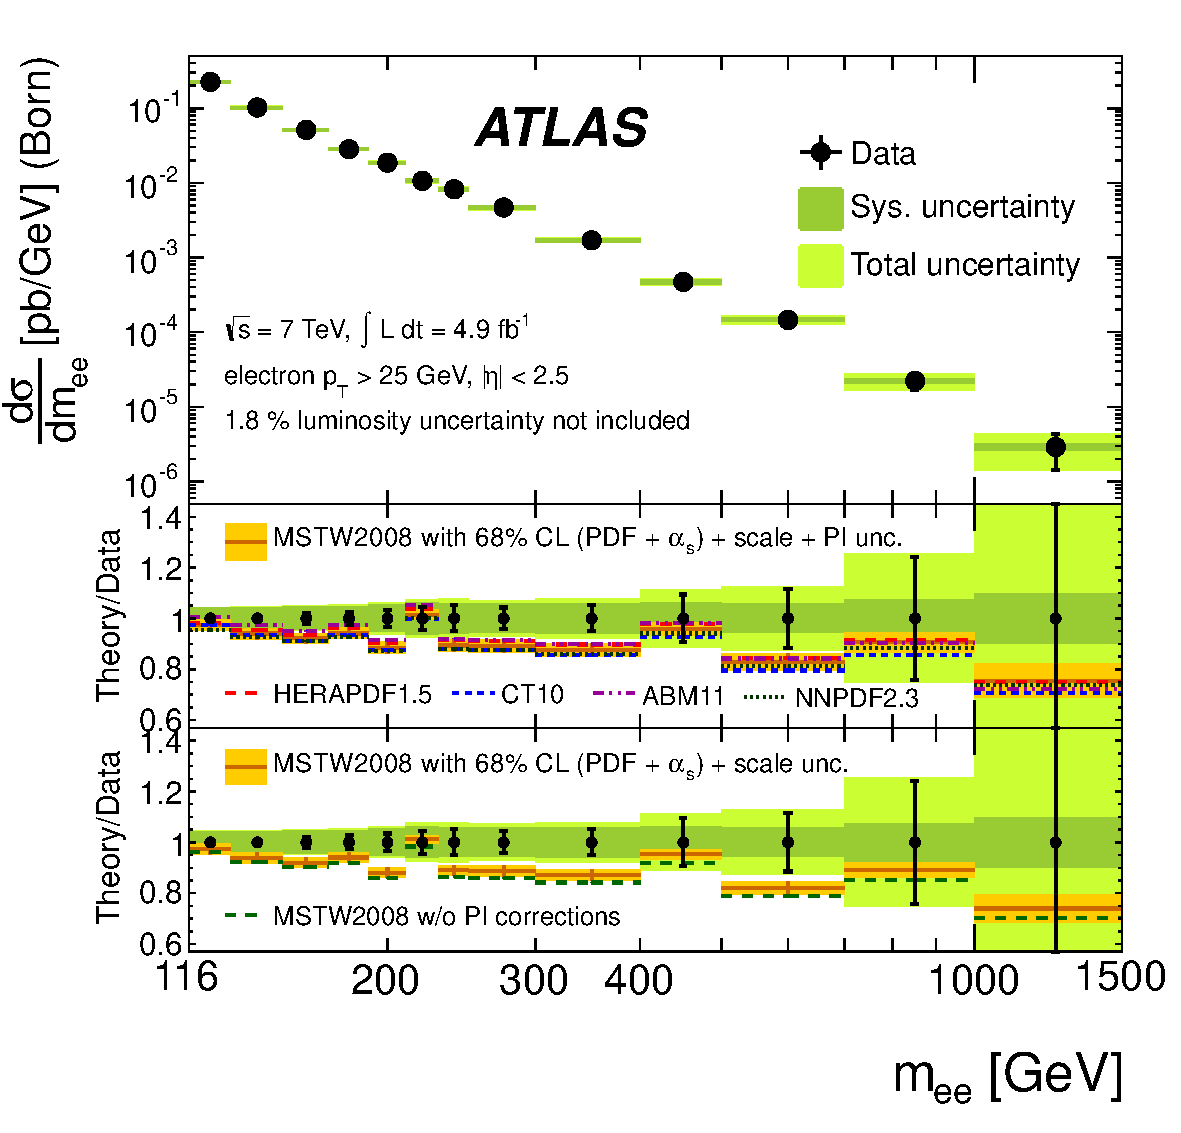
\includegraphics[height=0.3\textheight]{atlas_drellyan7tev}
    \caption{Measured differential cross-section at the Born level within the fiducial region (electron $p_T > 25$ GeV and $|\eta| < 2.5$) with statistical, systematic, and combined statistical and systematic (total) uncertainties, excluding the 1.8\% uncertainty on the luminosity. The measurement is compared to FEWZ 3.1 calculations at NNLO QCD with NLO electroweak corrections using the $G_{\mu}$ electroweak parameter scheme. The predictions include an additional small correction from single-boson production in which the final-state charged lepton radiates a real W or Z boson. On the left, in the upper ratio plot, the photon-induced (PI) corrections have been added to the predictions obtained from the MSTW2008, HERAPDF1.5, CT10, ABM11 and NNPDF2.3 NNLO PDFs, and for the MSTW2008 prediction the total uncertainty band arising from the PDF, $\alpha_s$, renormalisation and factorisation scale, and photon-induced uncertainties is drawn. The lower ratio plot shows the influence of the photon-induced corrections on the MSTW2008 prediction, the uncertainty band including only the PDF, $\alpha_s$ and scale uncertainties. On the right, the results are shown for a restricted range of $m_{ee}$.}
    \label{fig:atlas_drellyan7tev}
\end{figure}

\begin{figure}[p]
    \centering
    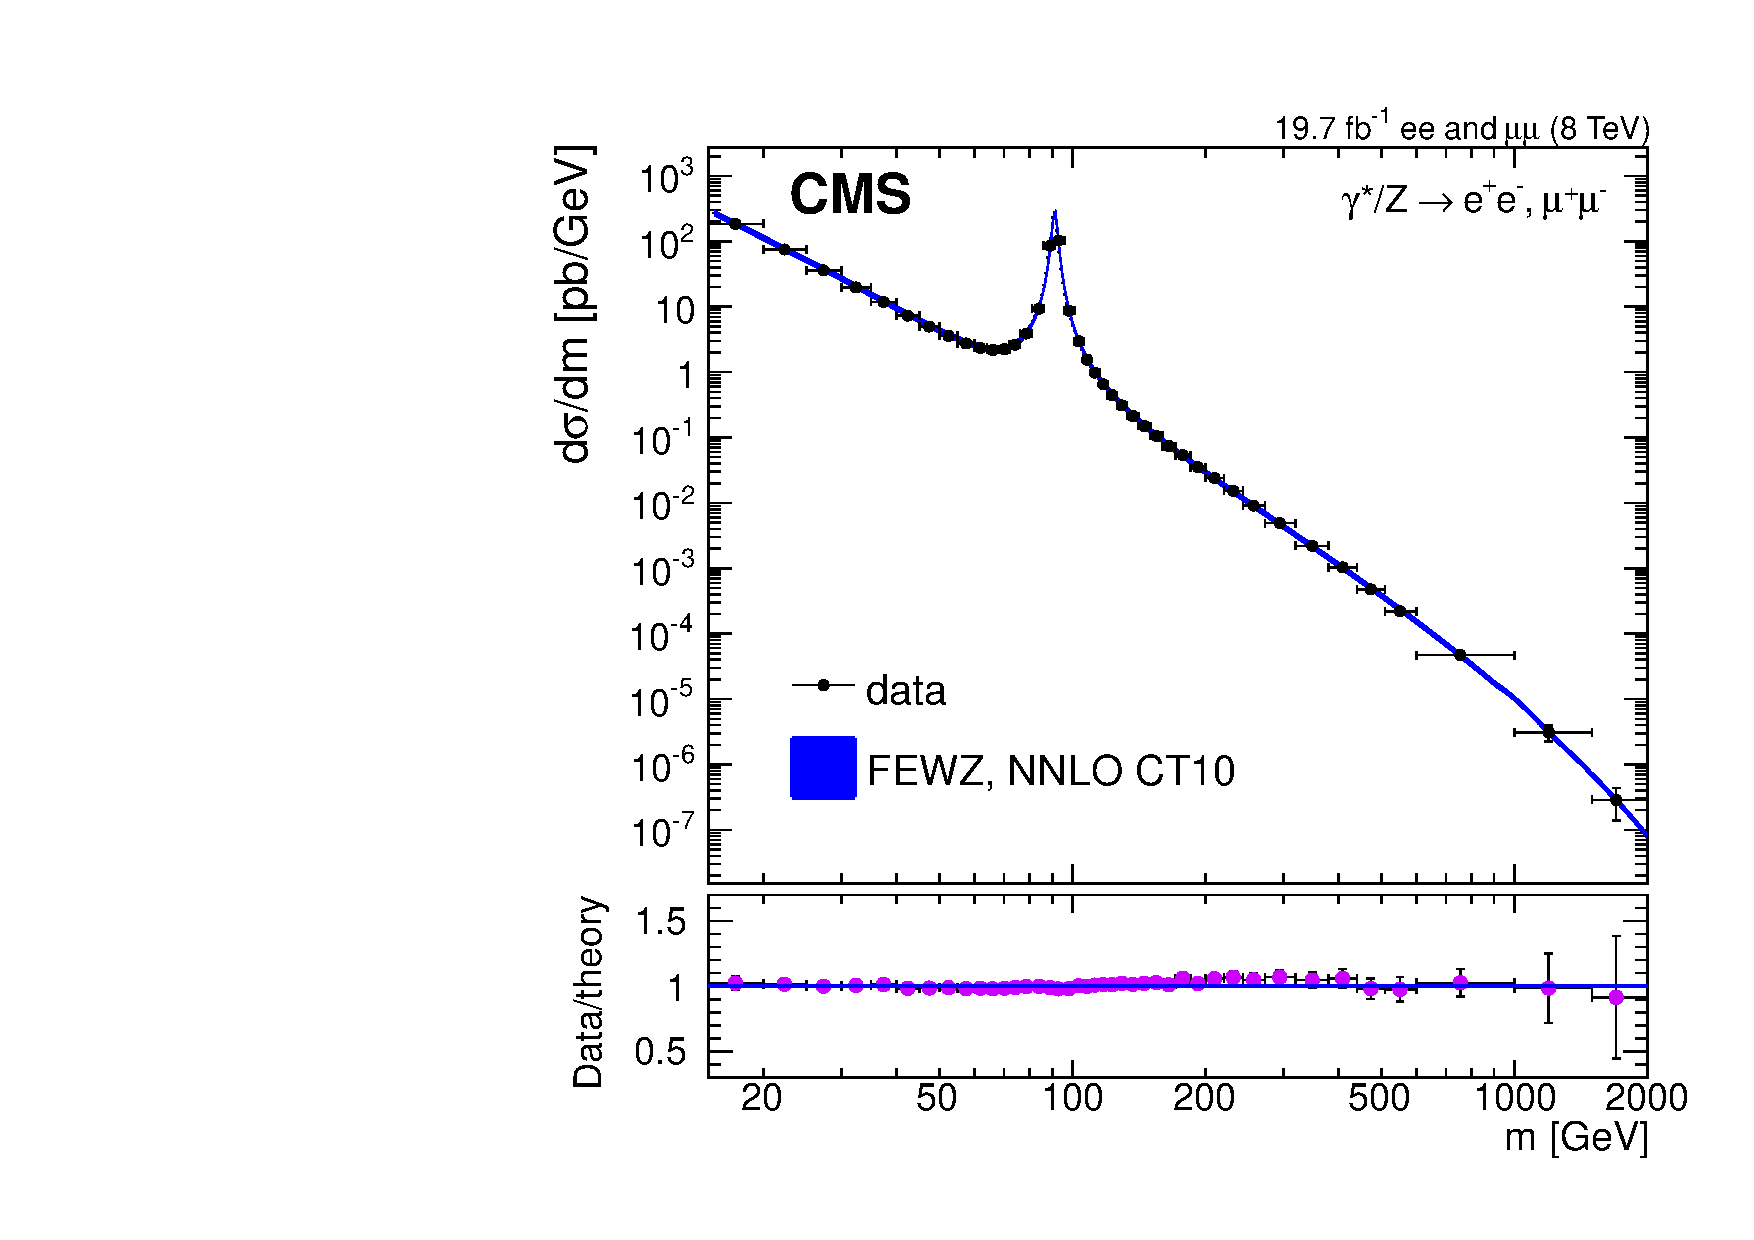
\includegraphics[height=0.3\textheight]{cms_drellyan8tev}
    \caption{}
    \label{fig:cms_drellyan8tev}
\end{figure}


\subsection{Inclusive di-boson production}

ATLAS Wgamma Zgamma 7 TeV~\cite{Aad:2013izg}

CMS Wgamma/Zgamma 7 TeV~\cite{Chatrchyan:2013fya}

CMS Znngamma 7 TeV~\cite{Chatrchyan:2013nda}

CMS Zgamma 8 TeV~\cite{Khachatryan:2015kea}


ATLAS simultaneous tt/WW/Z cross section 7 TeV~\cite{Aad:2014jra}

ATLAS WW 7 TeV~\cite{ATLAS:2012mec}

ATLAS $WW+WZ$ cross section 7 TeV~\cite{Aad:2014mda}

ATLAS WW 8 TeV~\cite{ATLAS-CONF-2014-033}

CMS WW2l2n 7 TeV~\cite{Chatrchyan:2013yaa}

CMS WWlnjj 7 TeV~\cite{Chatrchyan:2012bd}

CMS WW/ZZ 8 TeV~\cite{Chatrchyan:2013oev}

CMS WW2l2n 8 TeV (CMS-PAS-SMP-14-016, to be published)


ATLAS WZ 7 TeV~\cite{Aad:2012twa}

CMS VZ 8 TeV~\cite{Chatrchyan:2014aqa}

CMS WZ at 7+8 TeV (CMS-PAS-SMP-12-006, to be published)


ATLAS ZZ 7 TeV~\cite{Aad:2012awa}

CMS ZZ4l 8 TeV~\cite{Khachatryan:2014dia}

CMS ZZ4l 7 TeV~\cite{Chatrchyan:2012sga}

CMS ZZ2l2nu 7+8 TeV~\cite{Khachatryan:2015pba}

\subsection{Inclusive tri-boson production}

ATLAS $W\gamma\gamma$~\cite{Aad:2015uqa}

CMS WVgamma 8 TeV~\cite{Chatrchyan:2014bza}

\section{Exclusive boson production}
\subsection{Exclusive single boson production, vector-boson fusion}

ATLAS VBF Z 7 TeV~\cite{Aad:2014dta}

CMS VBF Z 7 TeV~\cite{Chatrchyan:2013jya}

CMS VBF Z 8 TeV~\cite{Khachatryan:2014dea}

\subsection{Exclusive di-boson production, vector-boson scattering}

ATLAS SSWW 8 TeV~\cite{Aad:2014zda}

CMS WWexcl 7 TeV~\cite{Chatrchyan:2013foa}

CMS SSWW 8 TeV~\cite{Khachatryan:2014sta}

\section{Electroweak (precision) tests of the standard model}
\subsection{Test of tri-boson vertex}

ATLAS Wgamma Zgamma 7 TeV~\cite{Aad:2013izg}

ATLAS WW 7 TeV~\cite{ATLAS:2012mec}

ATLAS $WW+WZ$ cross section 7 TeV~\cite{Aad:2014mda}

ATLAS WZ 7 TeV~\cite{Aad:2012twa}

CMS ZZ4l 8 TeV~\cite{Khachatryan:2014dia}

CMS ZZ4l 7 TeV~\cite{Chatrchyan:2012sga}

CMS WW2l2n 7 TeV~\cite{Chatrchyan:2013yaa}

CMS WWlnjj 7 TeV~\cite{Chatrchyan:2012bd}

CMS WW2l2n 8 TeV (CMS-PAS-SMP-14-016, to be published)

CMS Wgamma/Zgamma 7 TeV~\cite{Chatrchyan:2013fya}

CMS Znngamma 7 TeV~\cite{Chatrchyan:2013nda}

CMS Zgamma 8 TeV~\cite{Khachatryan:2015kea}

CMS ZZ2l2nu 7+8 TeV~\cite{Khachatryan:2015pba}

\subsection{Test of tetra-boson vertex}

ATLAS $W\gamma\gamma$ 8 TeV~\cite{Aad:2015uqa}

ATLAS SSWW 8 TeV~\cite{Aad:2014zda}

CMS WVgamma 8 TeV~\cite{Chatrchyan:2014bza}

CMS WWexcl 7 TeV~\cite{Chatrchyan:2013foa}

CMS SSWW 8 TeV~\cite{Khachatryan:2014sta}

\subsection{Z AFB and sin thetaW}

ATLAS weak mixing angle~\cite{Aad:2015uau}

CMS weak mixing angle~\cite{Chatrchyan:2011ya}

CMS Drell--Yan AFB 7 TeV~\cite{Chatrchyan:2012dc}

CMS Drell--Yan AFB 8 TeV (CMS-PAS-SMP-14-004, to be published)

\subsection{W mass}


\section{Summary}


ATLAS~\cite{Aad:2008zzm}
CDF~\cite{Abulencia:2005ix}
CMS~\cite{CMSdetector}
D0~\cite{Abazov:2005pn}
LHCb~\cite{Alves:2008zz}

CDF Z asymmetry muon~\cite{Aaltonen:2014loa}
CDF Z asymmetry electron~\cite{Aaltonen:2013wcp}
CDF W mass PRD~\cite{Aaltonen:2013vwa}
CDF W mass PRL~\cite{Aaltonen:2012bp}

D0 W asymmetry electron~\cite{Abazov:2013dsa}
D0 W asymmetry muon~\cite{Abazov:2013rja}
D0 W mass PRD~\cite{D0:2013jba}
D0 W mass PRL~\cite{Abazov:2012bv}

CDF+D0 W mass combination~\cite{Aaltonen:2013iut}

Snowmass electroweak~\cite{Baak:2013fwa}

Wmass PDF~\cite{Bozzi:2011ww}

\ack
Acknowledgments go here. 

\bibliographystyle{iopart-num}
\bibliography{ewkrun1_master}

\end{document}

